\documentclass[tikz,border=10pt]{standalone}
\usepackage{amsmath,amssymb}
\usepackage{tikz}
\usetikzlibrary{arrows.meta,positioning,shapes.geometric,calc,patterns,decorations.pathreplacing}

\definecolor{harvardcrimson}{RGB}{165,28,48}
\definecolor{ethblue}{RGB}{31,64,122}
\definecolor{petrol}{RGB}{0,122,135}
\definecolor{bronze}{RGB}{184,115,51}
\definecolor{darkslate}{RGB}{47,79,79}
\definecolor{lightgray}{RGB}{248,249,252}
\definecolor{bordergray}{RGB}{210,215,225}

\begin{document}
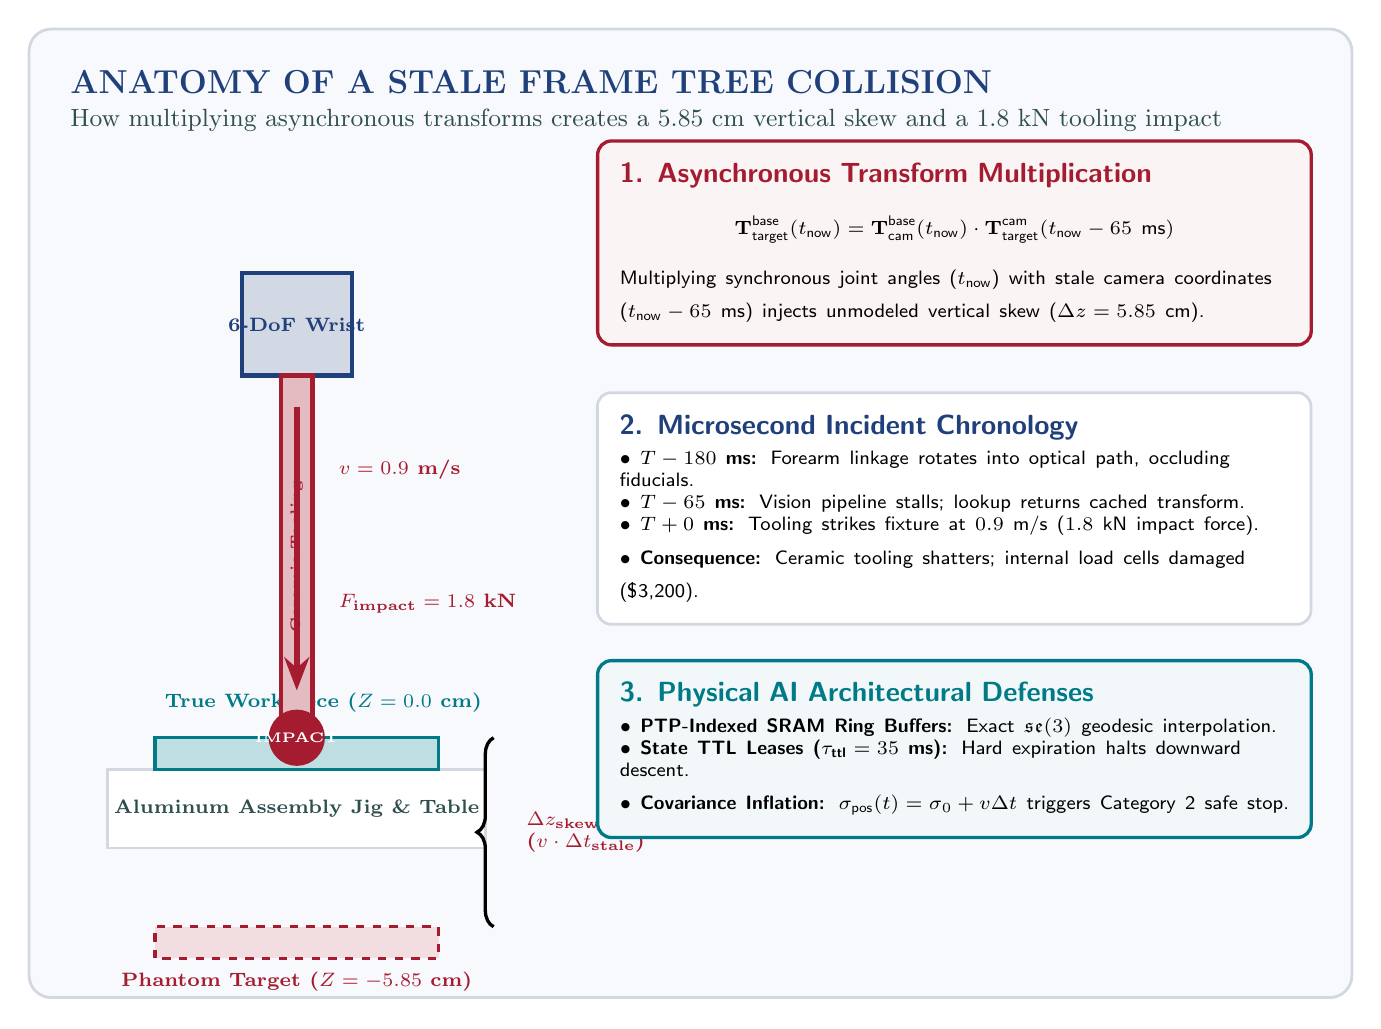
\begin{tikzpicture}[
    font=\sffamily,
    >=Stealth,
    node distance=1.5cm,
    box/.style={draw=bordergray, fill=white, rounded corners=5pt, line width=1pt, align=left, inner sep=8pt},
    alertbox/.style={draw=harvardcrimson, fill=harvardcrimson!5, rounded corners=5pt, line width=1.2pt, align=left, inner sep=8pt},
    safe/.style={draw=petrol, fill=petrol!5, rounded corners=5pt, line width=1.2pt, align=left, inner sep=8pt}
]

% Background Card
\draw[draw=bordergray, fill=lightgray, rounded corners=8pt, line width=1pt] (-0.8, -10.5) rectangle (16.0, 1.8);

% Title Banner
\node[anchor=north west, font=\bfseries\large, text=ethblue] at (-0.4, 1.4) {ANATOMY OF A STALE FRAME TREE COLLISION};
\node[anchor=north west, font=\small, text=darkslate] at (-0.4, 0.9) {How multiplying asynchronous transforms creates a $5.85\text{ cm}$ vertical skew and a $1.8\text{ kN}$ tooling impact};

% Left: Physical Kinematic Tree & Collision Geometry
\begin{scope}[shift={(0,0)}]
    % Optical Table & Jig
    \draw[fill=white, draw=bordergray, line width=1pt] (0.2,-8.6) rectangle (5.0,-7.6);
    \node[font=\scriptsize\bfseries, text=darkslate] at (2.6,-8.1) {Aluminum Assembly Jig \& Table};
    
    % PCB Workpiece (True Physical Position)
    \draw[fill=petrol!25, draw=petrol, line width=1.2pt] (0.8,-7.6) rectangle (4.4,-7.2);
    \node[font=\scriptsize\bfseries, text=petrol, anchor=south west] at (0.8,-7.0) {True Workpiece ($Z = 0.0\text{ cm}$)};

    % Phantom Target (Calculated Position due to 65ms Stale Transform)
    \draw[dashed, fill=harvardcrimson!15, draw=harvardcrimson, line width=1.2pt] (0.8,-10.0) rectangle (4.4,-9.6);
    \node[font=\scriptsize\bfseries, text=harvardcrimson, anchor=north] at (2.6,-10.05) {Phantom Target ($Z = -5.85\text{ cm}$)};
    
    % Skew Measurement Brace
    \draw[decorate, decoration={brace, amplitude=6pt, mirror}, text=harvardcrimson, line width=1.2pt] (5.1,-7.2) -- (5.1,-9.6)
        node[midway, right=8pt, font=\scriptsize\bfseries, text=harvardcrimson, align=left] {$\Delta z_{\text{skew}} = 5.85\text{ cm}$\\($v \cdot \Delta t_{\text{stale}}$)};

    % Robot Arm Wrist
    \draw[fill=ethblue!20, draw=ethblue, line width=1.5pt] (1.9,-2.6) rectangle (3.3,-1.3);
    \node[font=\scriptsize\bfseries, text=ethblue] at (2.6,-1.95) {6-DoF Wrist};
    
    % Vacuum Tooling
    \draw[fill=harvardcrimson!30, draw=harvardcrimson, line width=1.5pt] (2.4,-7.2) rectangle (2.8,-2.6);
    \node[font=\tiny\bfseries, text=harvardcrimson, rotate=90] at (2.6,-4.9) {Ceramic Tooling};
    
    % Impact Force Starburst / Circle
    \draw[fill=harvardcrimson, text=white, draw=harvardcrimson] (2.6,-7.2) circle (0.35);
    \node[font=\tiny\bfseries, text=white] at (2.6,-7.2) {IMPACT};
    
    % Velocity & Force vectors
    \draw[->, line width=2pt, harvardcrimson] (2.6,-3.0) -- (2.6,-6.6);
    \node[font=\scriptsize\bfseries, text=harvardcrimson, right=6pt] at (2.8,-3.8) {$v = 0.9\text{ m/s}$};
    \node[font=\scriptsize\bfseries, text=harvardcrimson, right=6pt] at (2.8,-5.5) {$F_{\text{impact}} = 1.8\text{ kN}$};
\end{scope}

% Right: Telemetry & Architectural Cause/Remedy (Clean Vertical Stacking)
\begin{scope}[shift={(6.4, 0.4)}]
    % Box 1: The Root Cause
    \node[alertbox, text width=8.5cm, anchor=north west] at (0, 0) {
        \textbf{\color{harvardcrimson} 1. Asynchronous Transform Multiplication}\\[3pt]
        \scriptsize
        $$\mathbf{T}_{\text{target}}^{\text{base}}(t_{\text{now}}) = \mathbf{T}_{\text{cam}}^{\text{base}}(t_{\text{now}}) \cdot \mathbf{T}_{\text{target}}^{\text{cam}}(t_{\text{now}} - 65\text{ ms})$$
        Multiplying synchronous joint angles ($t_{\text{now}}$) with stale camera coordinates ($t_{\text{now}}-65\text{ ms}$) injects unmodeled vertical skew ($\Delta z = 5.85\text{ cm}$).
    };

    % Box 2: The Timeline
    \node[box, text width=8.5cm, anchor=north west] at (0, -3.2) {
        \textbf{\color{ethblue} 2. Microsecond Incident Chronology}\\[3pt]
        \scriptsize\raggedright
        $\bullet$ \textbf{$T - 180\text{ ms}$:} Forearm linkage rotates into optical path, occluding fiducials.\\
        $\bullet$ \textbf{$T - 65\text{ ms}$:} Vision pipeline stalls; lookup returns cached transform.\\
        $\bullet$ \textbf{$T + 0\text{ ms}$:} Tooling strikes fixture at $0.9\text{ m/s}$ ($1.8\text{ kN}$ impact force).\\
        $\bullet$ \textbf{Consequence:} Ceramic tooling shatters; internal load cells damaged (\$3,200).
    };

    % Box 3: Architectural Defense
    \node[safe, text width=8.5cm, anchor=north west] at (0, -6.6) {
        \textbf{\color{petrol} 3. Physical AI Architectural Defenses}\\[3pt]
        \scriptsize\raggedright
        $\bullet$ \textbf{PTP-Indexed SRAM Ring Buffers:} Exact $\mathfrak{se}(3)$ geodesic interpolation.\\
        $\bullet$ \textbf{State TTL Leases ($\tau_{\text{ttl}} = 35\text{ ms}$):} Hard expiration halts downward descent.\\
        $\bullet$ \textbf{Covariance Inflation:} $\sigma_{\text{pos}}(t) = \sigma_0 + v\Delta t$ triggers Category 2 safe stop.
    };
\end{scope}

\end{tikzpicture}
\end{document}
